\chapter{Architecture Design}
\label{chap:architecture_design}

\section*{Introduction}
This chapter provides a detailed exploration of the system architecture, which is designed to be modular, scalable, and secure. Key components include the integration of Large Language Models (LLMs), the implementation of a highly specialized Retrieval-Augmented Generation (RAG) architecture, modern frontend and backend architecture used, the log systesm used in this project.

\pagebreak

\section{Detailed Component Architecture}

The platform's backend architecture follows a highly decoupled approach using FastAPI. This ensures that services are modular, asynchronous, and scalable.
\subsection{Backend Design}
\begin{itemize}


\item \textbf{Data Management:} Uses PostgreSQL (\texttt{asyncpg}/SQLAlchemy) for highly responsive data storage. It enforces strict tenant isolation via Row-Level Security (RLS), storing user files and projects in dedicated, authenticated directories with zero public exposure.

\item \textbf{System Logging \& Telemetry:} An asynchronous JSON logging system tracks all API, database, and RAG operations. It ensures security by scrubbing sensitive data via Regex, and optimizes storage through nightly \texttt{.gz} compression with an automated 30-day deletion policy.

\IfFileExists{Figures/logArch.png}{
    \begin{figure}[H]
        \centering
        \includegraphics[width=0.8\textwidth]{Figures/logArch.png}
        \caption{Architecture of the Rotating JSON Log System}
        \label{fig:log_system}
    \end{figure}
}{}

\item \textbf{Authentication \& APIs:} \textbf{Clerk} handles secure Identity and Access Management via clerk, which the backend strictly verifies to enforce data ownership. A fully asynchronous FastAPI layer, auto-documented via Swagger, orchestrates all internal routing and external AI integrations (Gemini, OpenAI, LaTeXLite).

\IfFileExists{Figures/backend.png}{
    \begin{figure}[H]
        \centering
        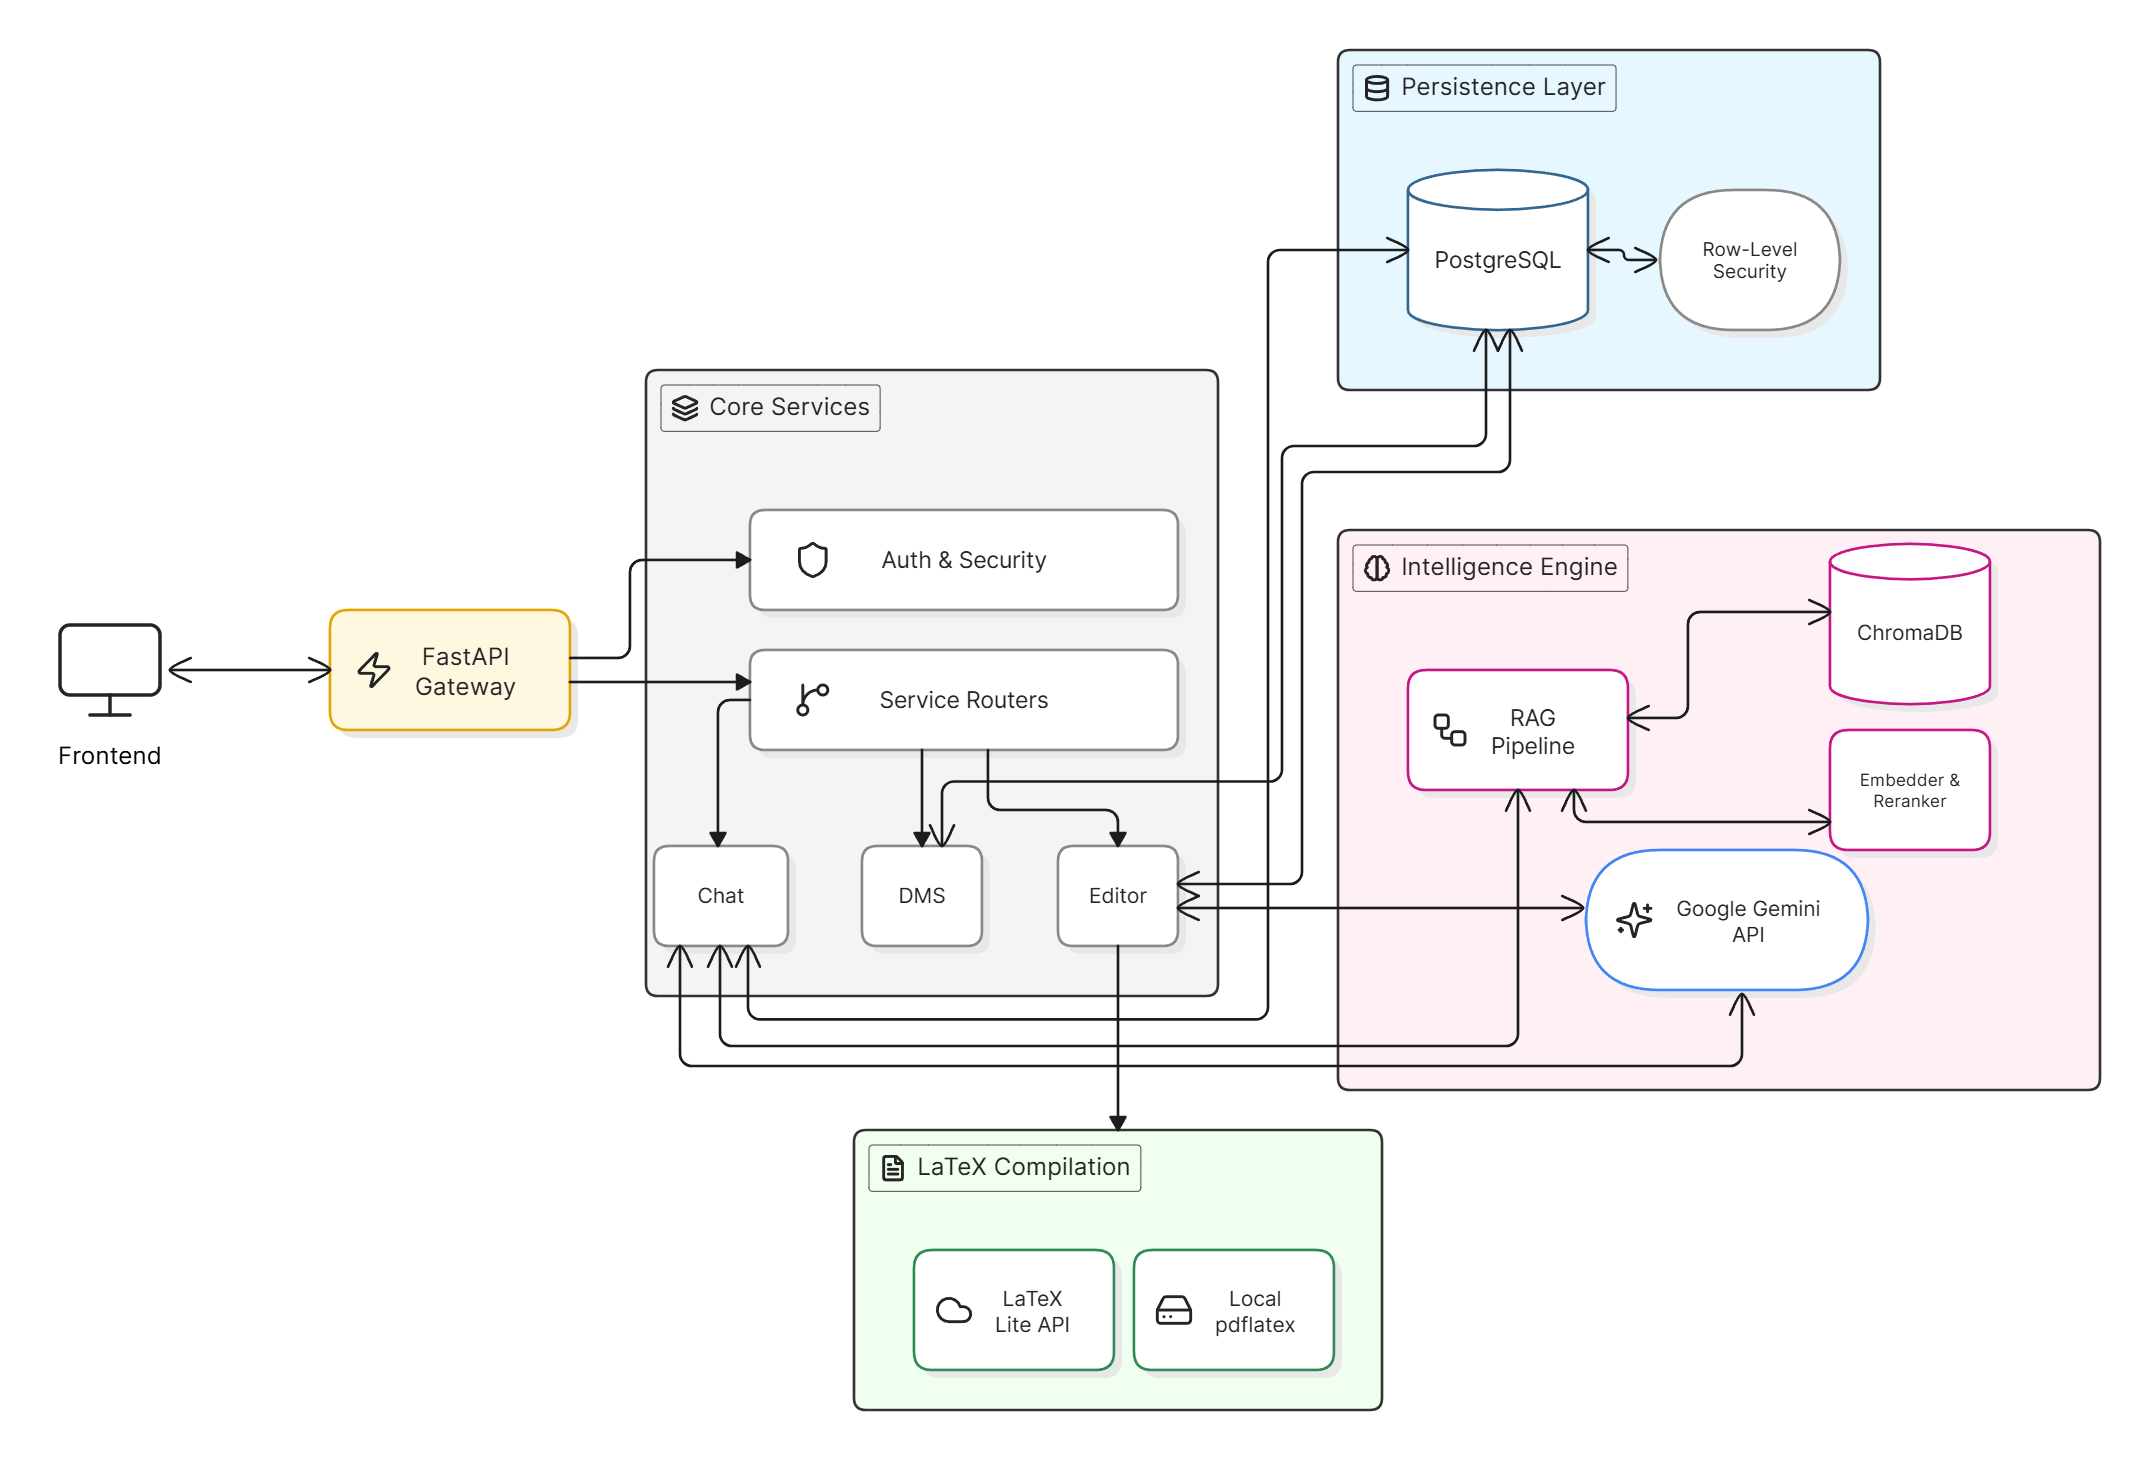
\includegraphics[width=0.8\textwidth]{Figures/backend.png}
        \caption{Detailed Backend Component Architecture}
        \label{fig:backend_arch}
    \end{figure}
}{}
\end{itemize}

\newpage
\section{RAG Architecture \& Intelligence Pipeline}

Our Retrieval-Augmented Generation (RAG) architecture is divided into two distinct, asynchronous phases to maximize accuracy and efficiently handle the morphological complexities of Moroccan legal documents.

\subsection{Phase 1: Offline Ingestion \& Storage}
The ingestion process begins by processing raw legal PDFs through \texttt{PyMuPDF} and \texttt{pdf2image}. These extracted images are routed to a Vision-Language Model (\textbf{GPT-4o Vision}) instructed by a strict, domain-specific prompt. This prompt forces the model to filter out administrative noise (such as repetitive headers, dates, and stamps) and autonomously structure the text using precise XML tags (\texttt{<chunk>} and \texttt{<table>}). 

A custom Python parser then segments this output. The text segments are mathematically embedded using the multilingual \texttt{BAAI/bge-m3} model and indexed securely in a \textbf{ChromaDB} vector store. Crucially, to optimize retrieval and prevent token overflow, only the descriptive titles of tables are embedded, while the full Markdown table structures are preserved securely within the payload metadata.

\subsection{Phase 2: Online Retrieval \& Generation}
During a live chat session, the user's query is intercepted and embedded using the same \texttt{BAAI/bge-m3} model. The system executes a high-speed cosine similarity search against ChromaDB, retrieving the Top 20 most mathematically relevant chunks. 

Because raw vector similarity can lack deep semantic nuance, these 20 chunks are passed through a Cross-Encoder neural network (\texttt{BAAI/bge-reranker-v2-m3}). The reranker evaluates the logical relationship between the query and each chunk, isolating the absolute Top 5 most relevant pieces of context. Finally, this highly refined context is assembled into a strict Arabic system prompt and dispatched to \textbf{Google Gemini 2.5 Flash}, which generates the final, hallucination-free legal response.

\IfFileExists{image.png}{
    \begin{figure}[H]
        \centering
        
\includegraphics[width=0.6\textwidth]{image.png}
        \caption{RAG Pipeline Execution Architecture}
        \label{fig:rag_arch}
    \end{figure}
}{}

\newpage
\section{Frontend Design}

The frontend is a Multiple Page Application (MPA) built using \textbf{React}. It employs a modular component architecture and a clean user interface. the color palette and typography (fonst) are inspired by the \textbf{Ollama} platform, while the conversational interface mirrors the intuitive layout of \textbf{Google Gemini}. Furthermore, the document editing workspace takes structural cues from \textbf{Overleaf} and the \textbf{Antigravity} AI coding tool, paired with a file management system that replicates the seamless, drag-and-drop experience of a native desktop file explorer. 

\subsection{Application Routing Tree (Sitemap)}
The application leverages \texttt{react-router-dom} to manage client-side navigation seamlessly without reloading the browser. The route structure is organized as follows:

\begin{verbatim}
/ (Root)
|-- /sign-in                  -> Authentication Portal (Clerk)
|-- /sign-up                  -> Registration Portal (Clerk)
|-- /                         -> Landing Page (Public overview & features)
|
|-- /chat                     -> Main AI Interface
|   |-- /chat/:id             -> Specific AI Conversation Thread
|
|-- /database                 -> Document Management System (DMS)
|                                (Virtual folders, upload, pagination, sorting)
|
|-- /editor                   -> Workspace for LaTeX Generation
|   |-- /editor/:id           -> Split-Screen Editor (Code / PDF Viewer / AI)
\end{verbatim}

\subsection{UI and Prototyping}

During the initial design phase, we utilized \textbf{Excalidraw} to draft the UI/UX wireframes and conceptualize the platform's layout. The primary objective of these mockups was to bridge the gap between the complex backend architecture and the end-user. By designing an intuitive, accessible, and highly visual interface, we ensure that users can effortlessly leverage all the advanced backend functionalities (such as the RAG pipeline and LaTeX compiler), thereby significantly enhancing the overall user experience.

The following figures illustrate the low-fidelity wireframes created to map out the user journeys across the platform's core modules.

\IfFileExists{Figures/landingPage.png}{
    \begin{figure}[H]
        \centering
        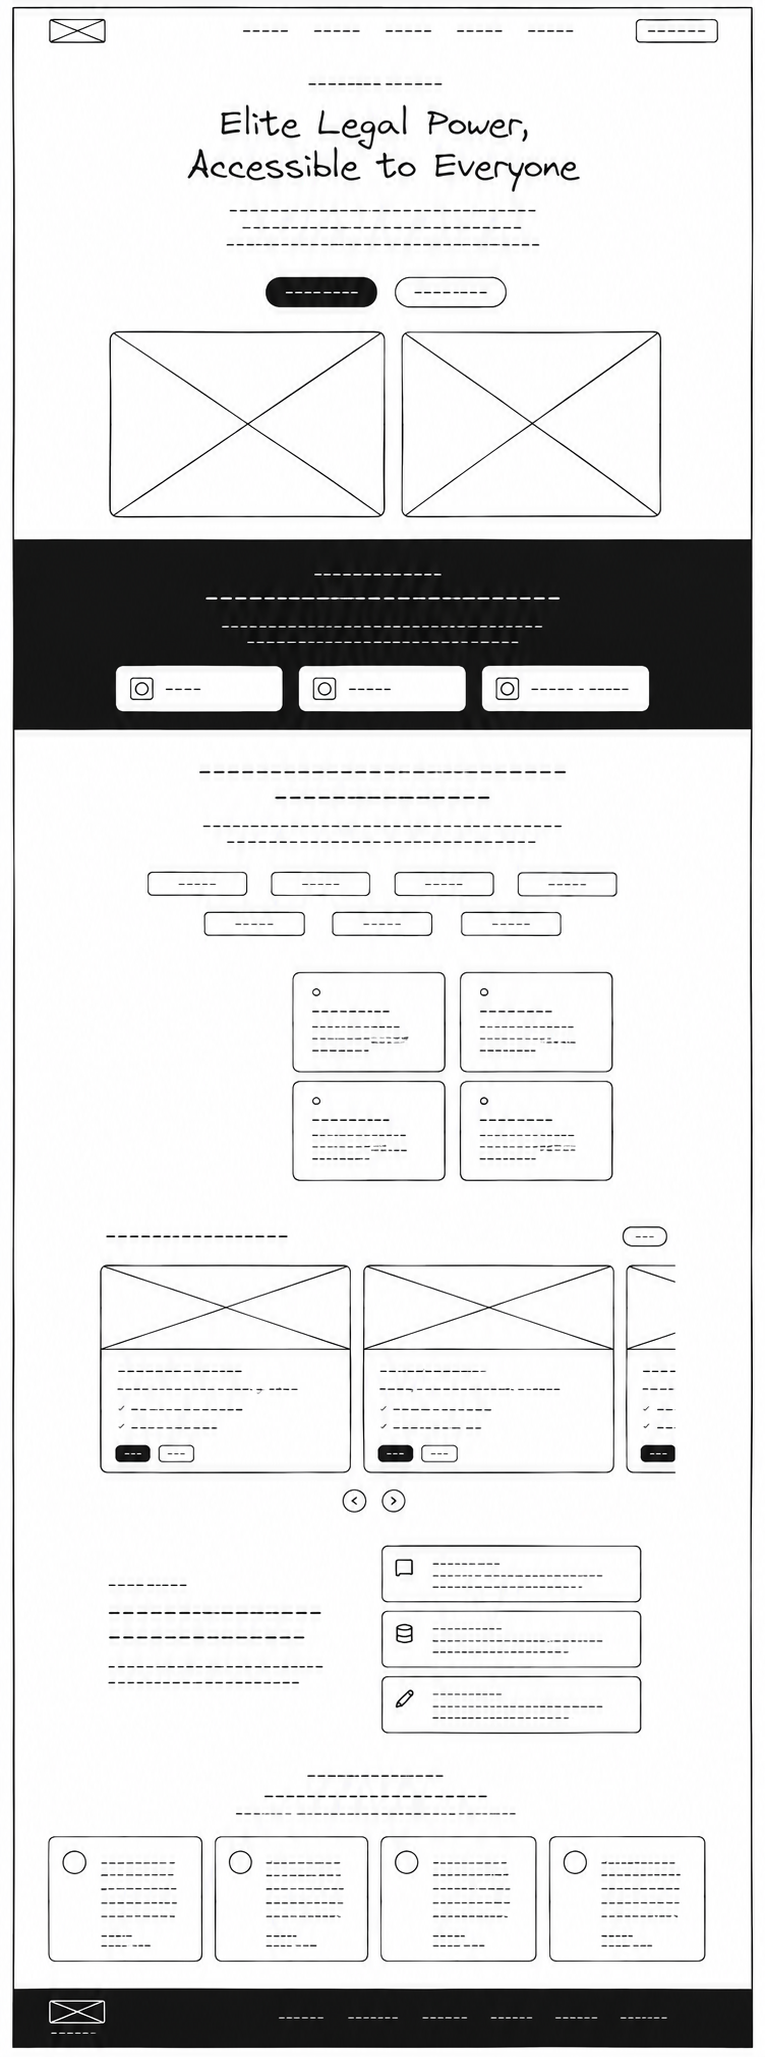
\includegraphics[width=0.55\textwidth]{Figures/landingPage.png}
        \caption{Wireframe mockup of the Public Landing Page}
        \label{fig:wireframe_landing}
    \end{figure}
}{}

\vspace{0.5cm}

\IfFileExists{Figures/chatpage.png}{
    \begin{figure}[H]
        \centering
        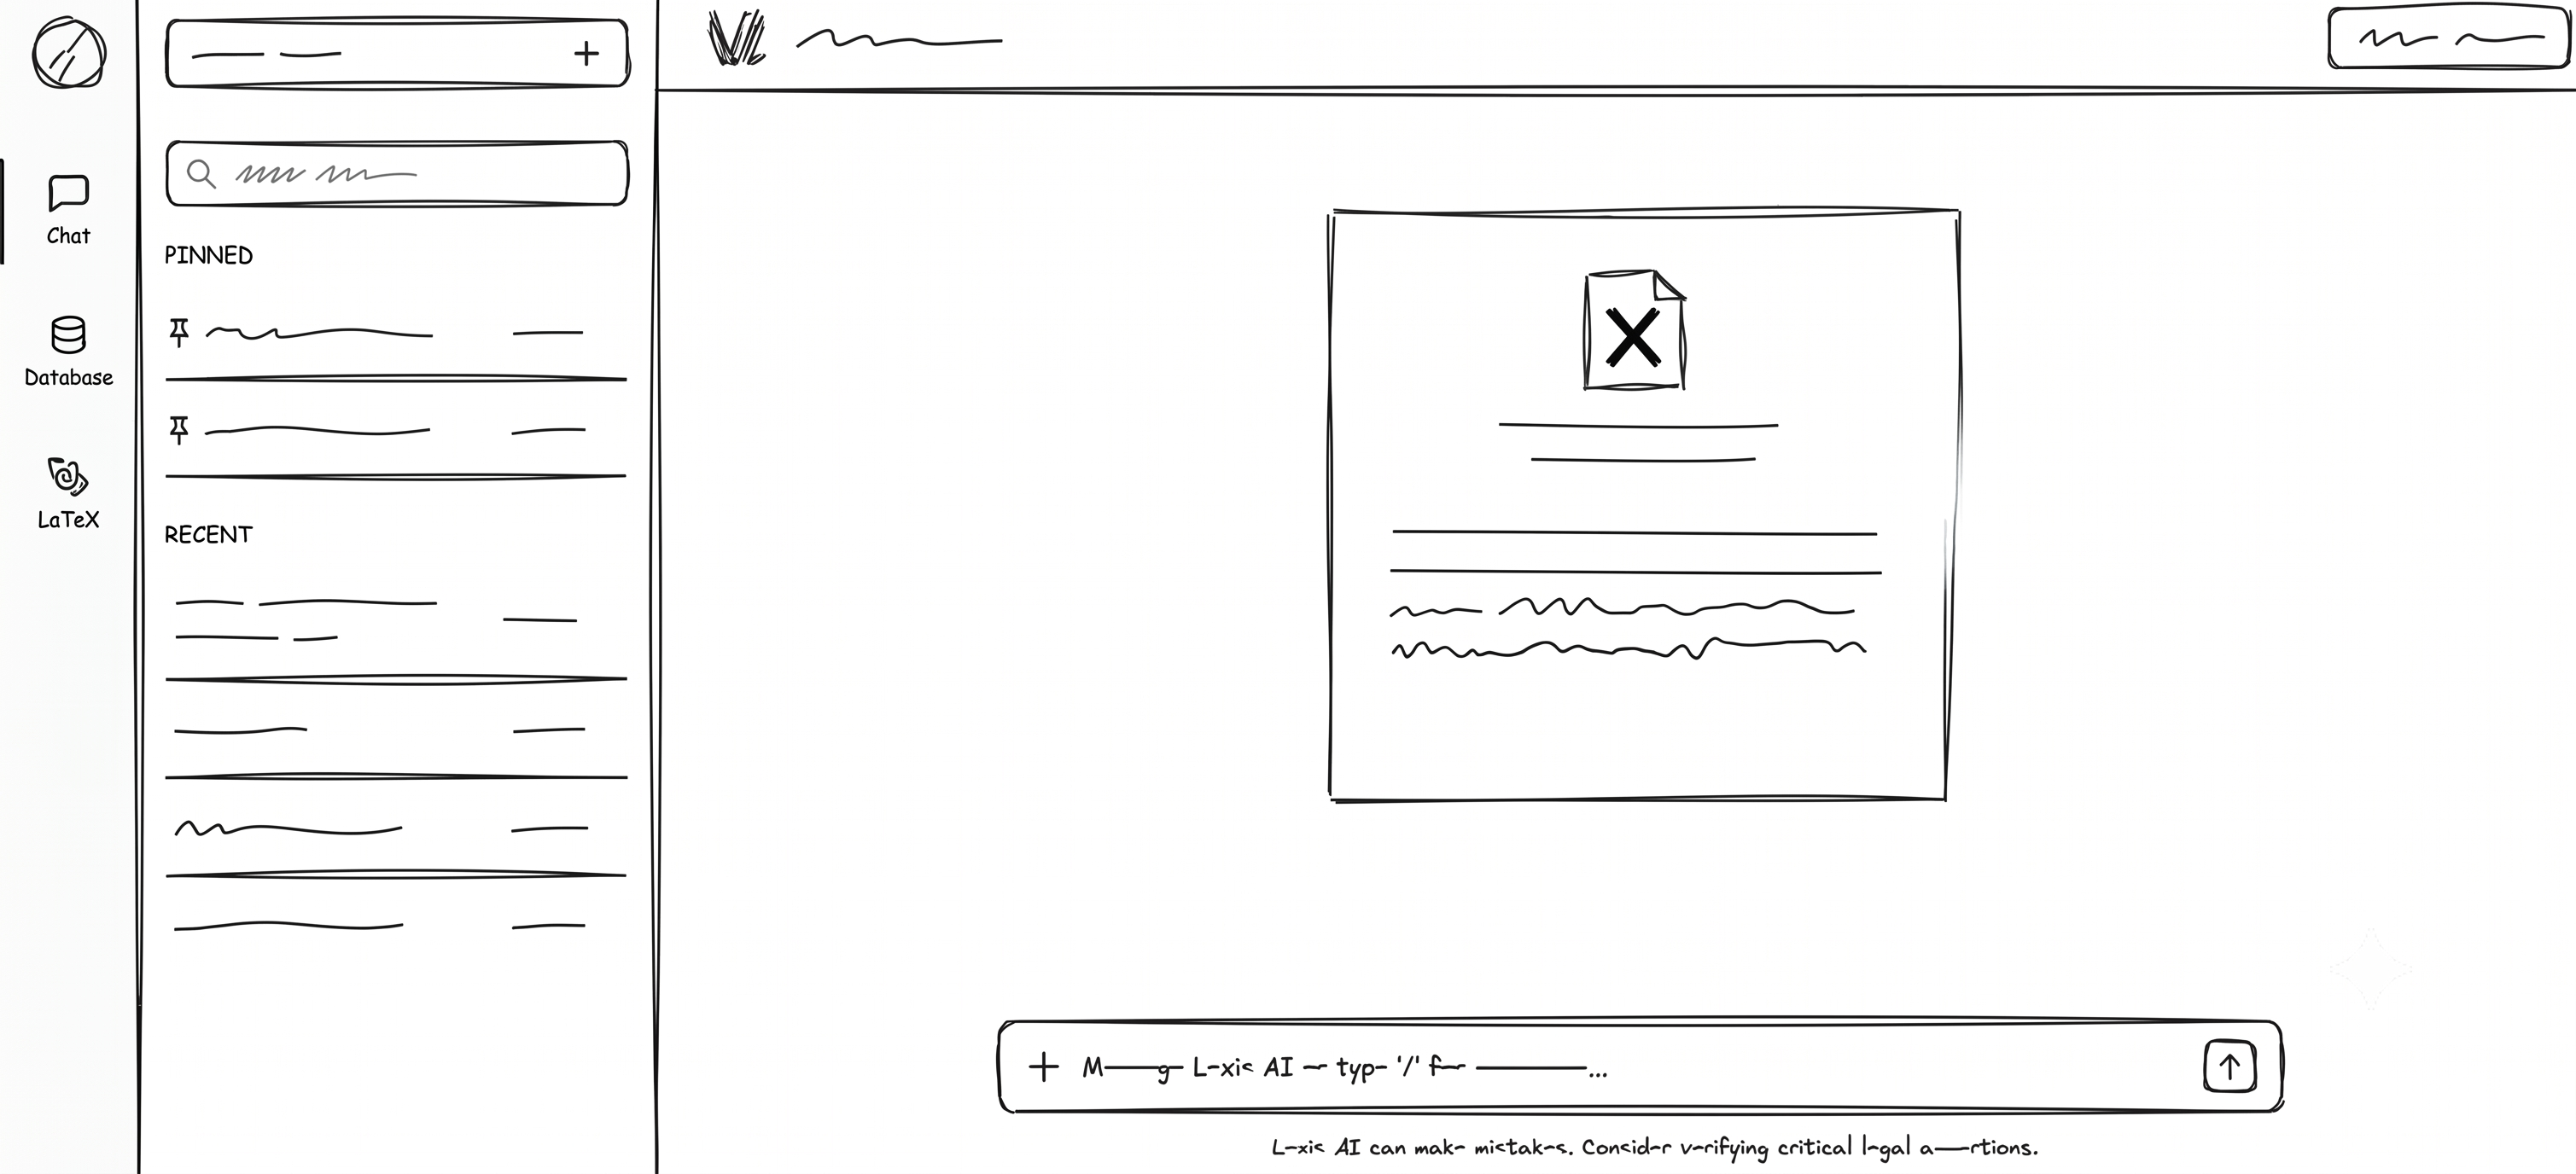
\includegraphics[width=0.9\textwidth]{Figures/chatpage.png}
        \caption{Wireframe mockup of the Main AI Chat Interface}
        \label{fig:wireframe_chat}
    \end{figure}
}{}

\vspace{0.5cm}

\IfFileExists{Figures/latexPage.png}{
    \begin{figure}[H]
        \centering
        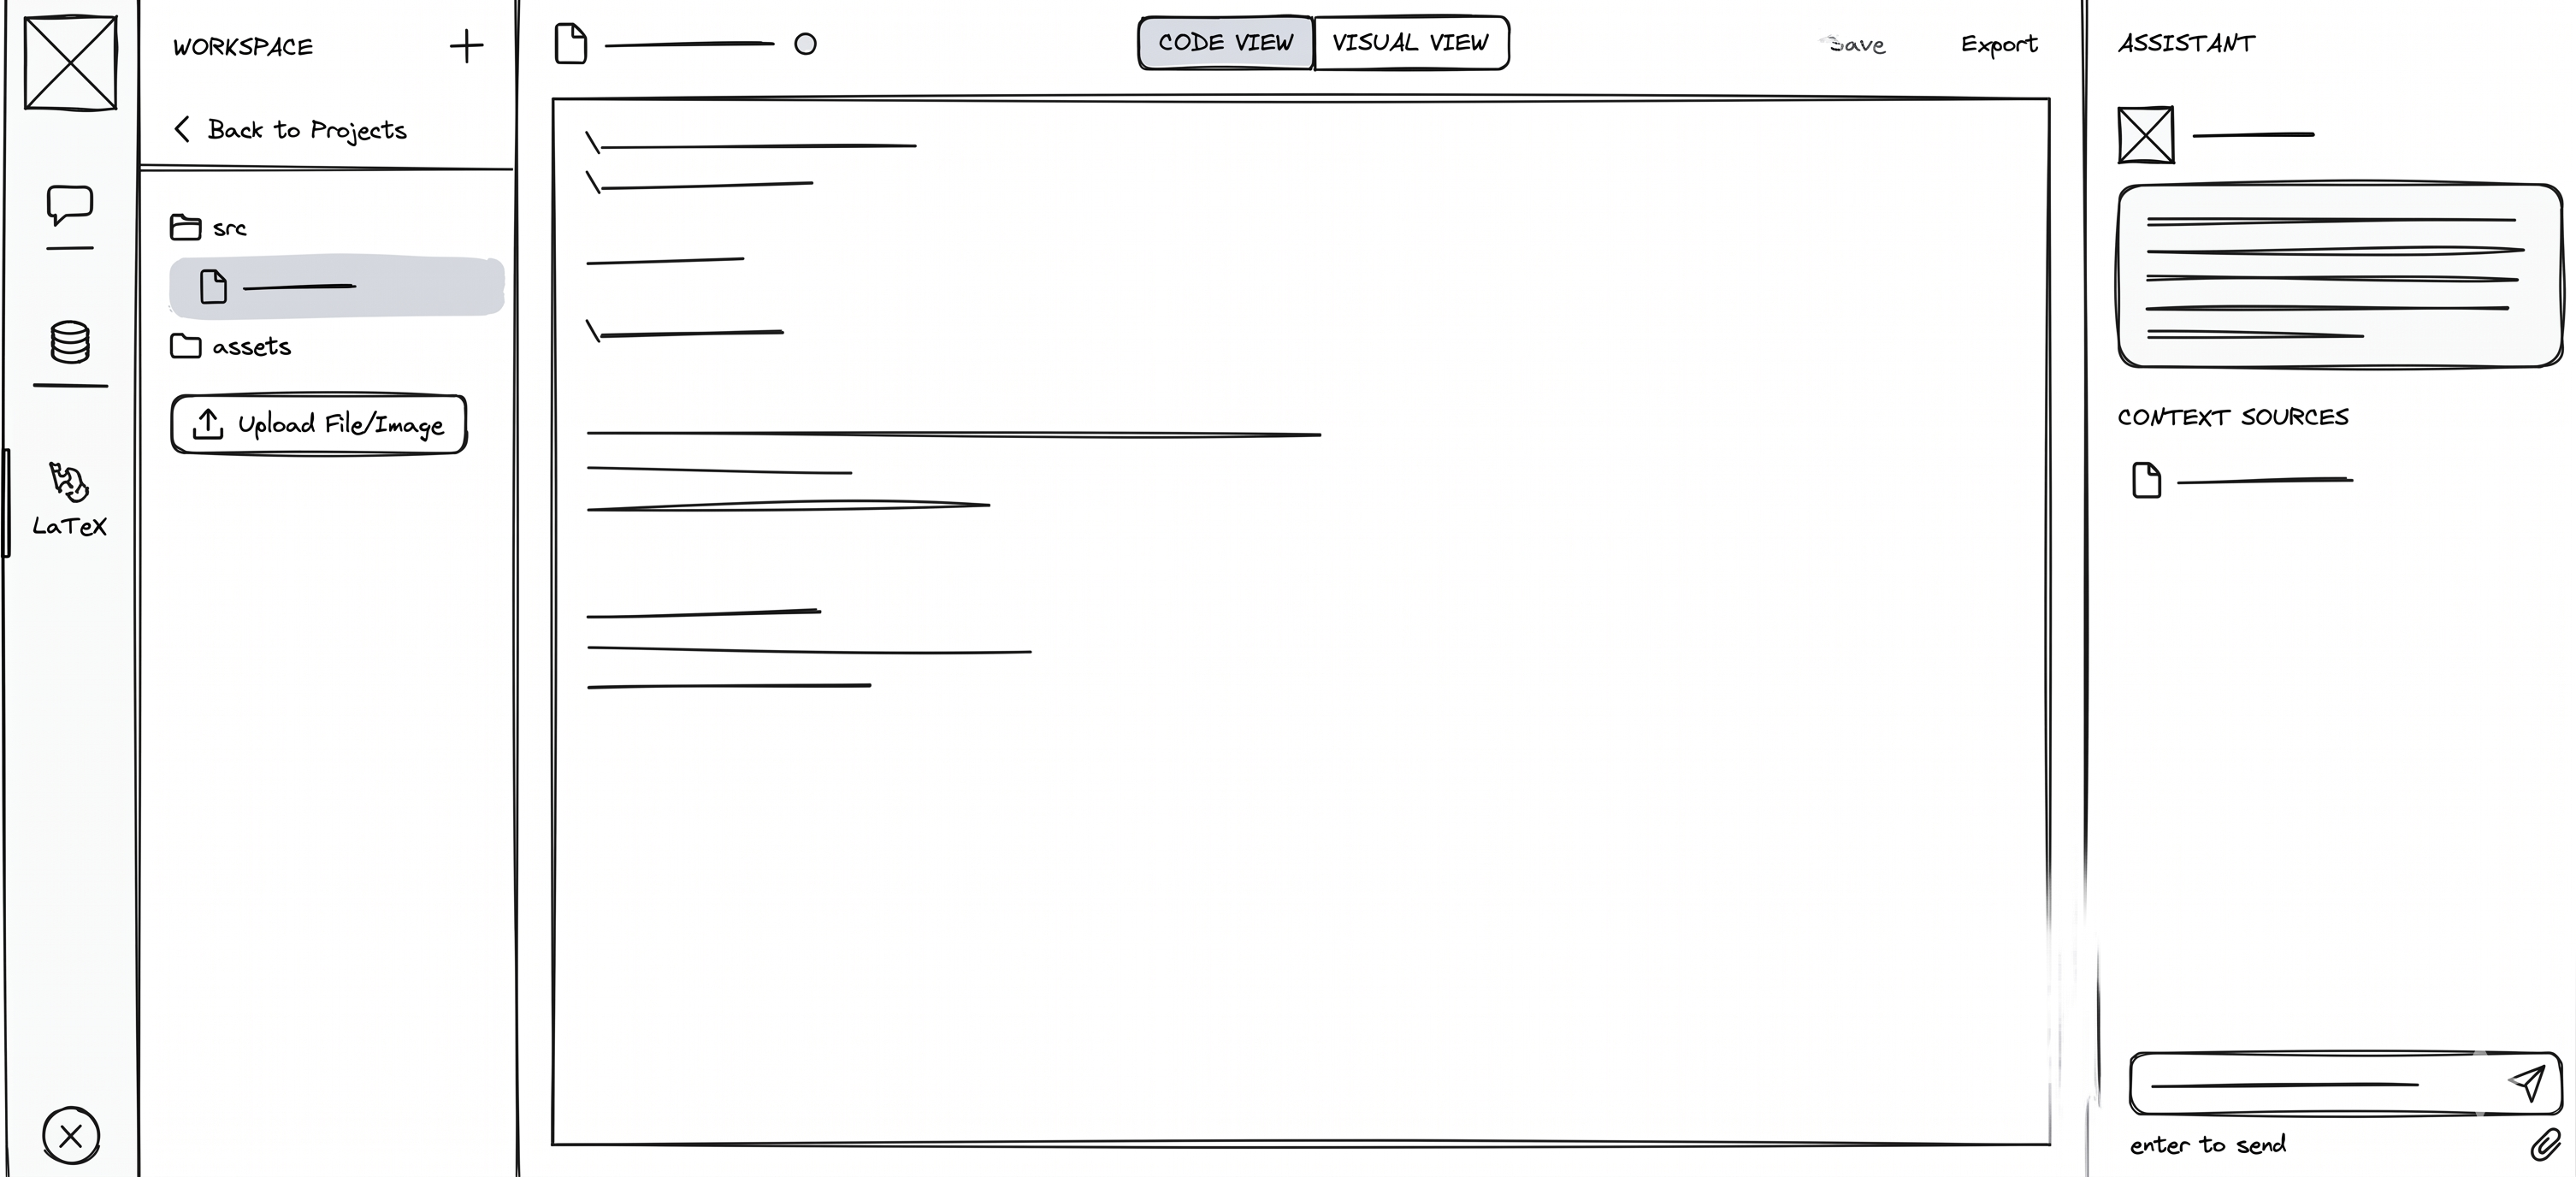
\includegraphics[width=0.9\textwidth]{Figures/latexPage.png}
        \caption{Wireframe mockup of the Split-Screen LaTeX Editor Workspace}
        \label{fig:wireframe_latex}
    \end{figure}
}{}

\vspace{0.5cm}

\IfFileExists{Figures/fileUploads.png}{
    \begin{figure}[H]
        \centering
        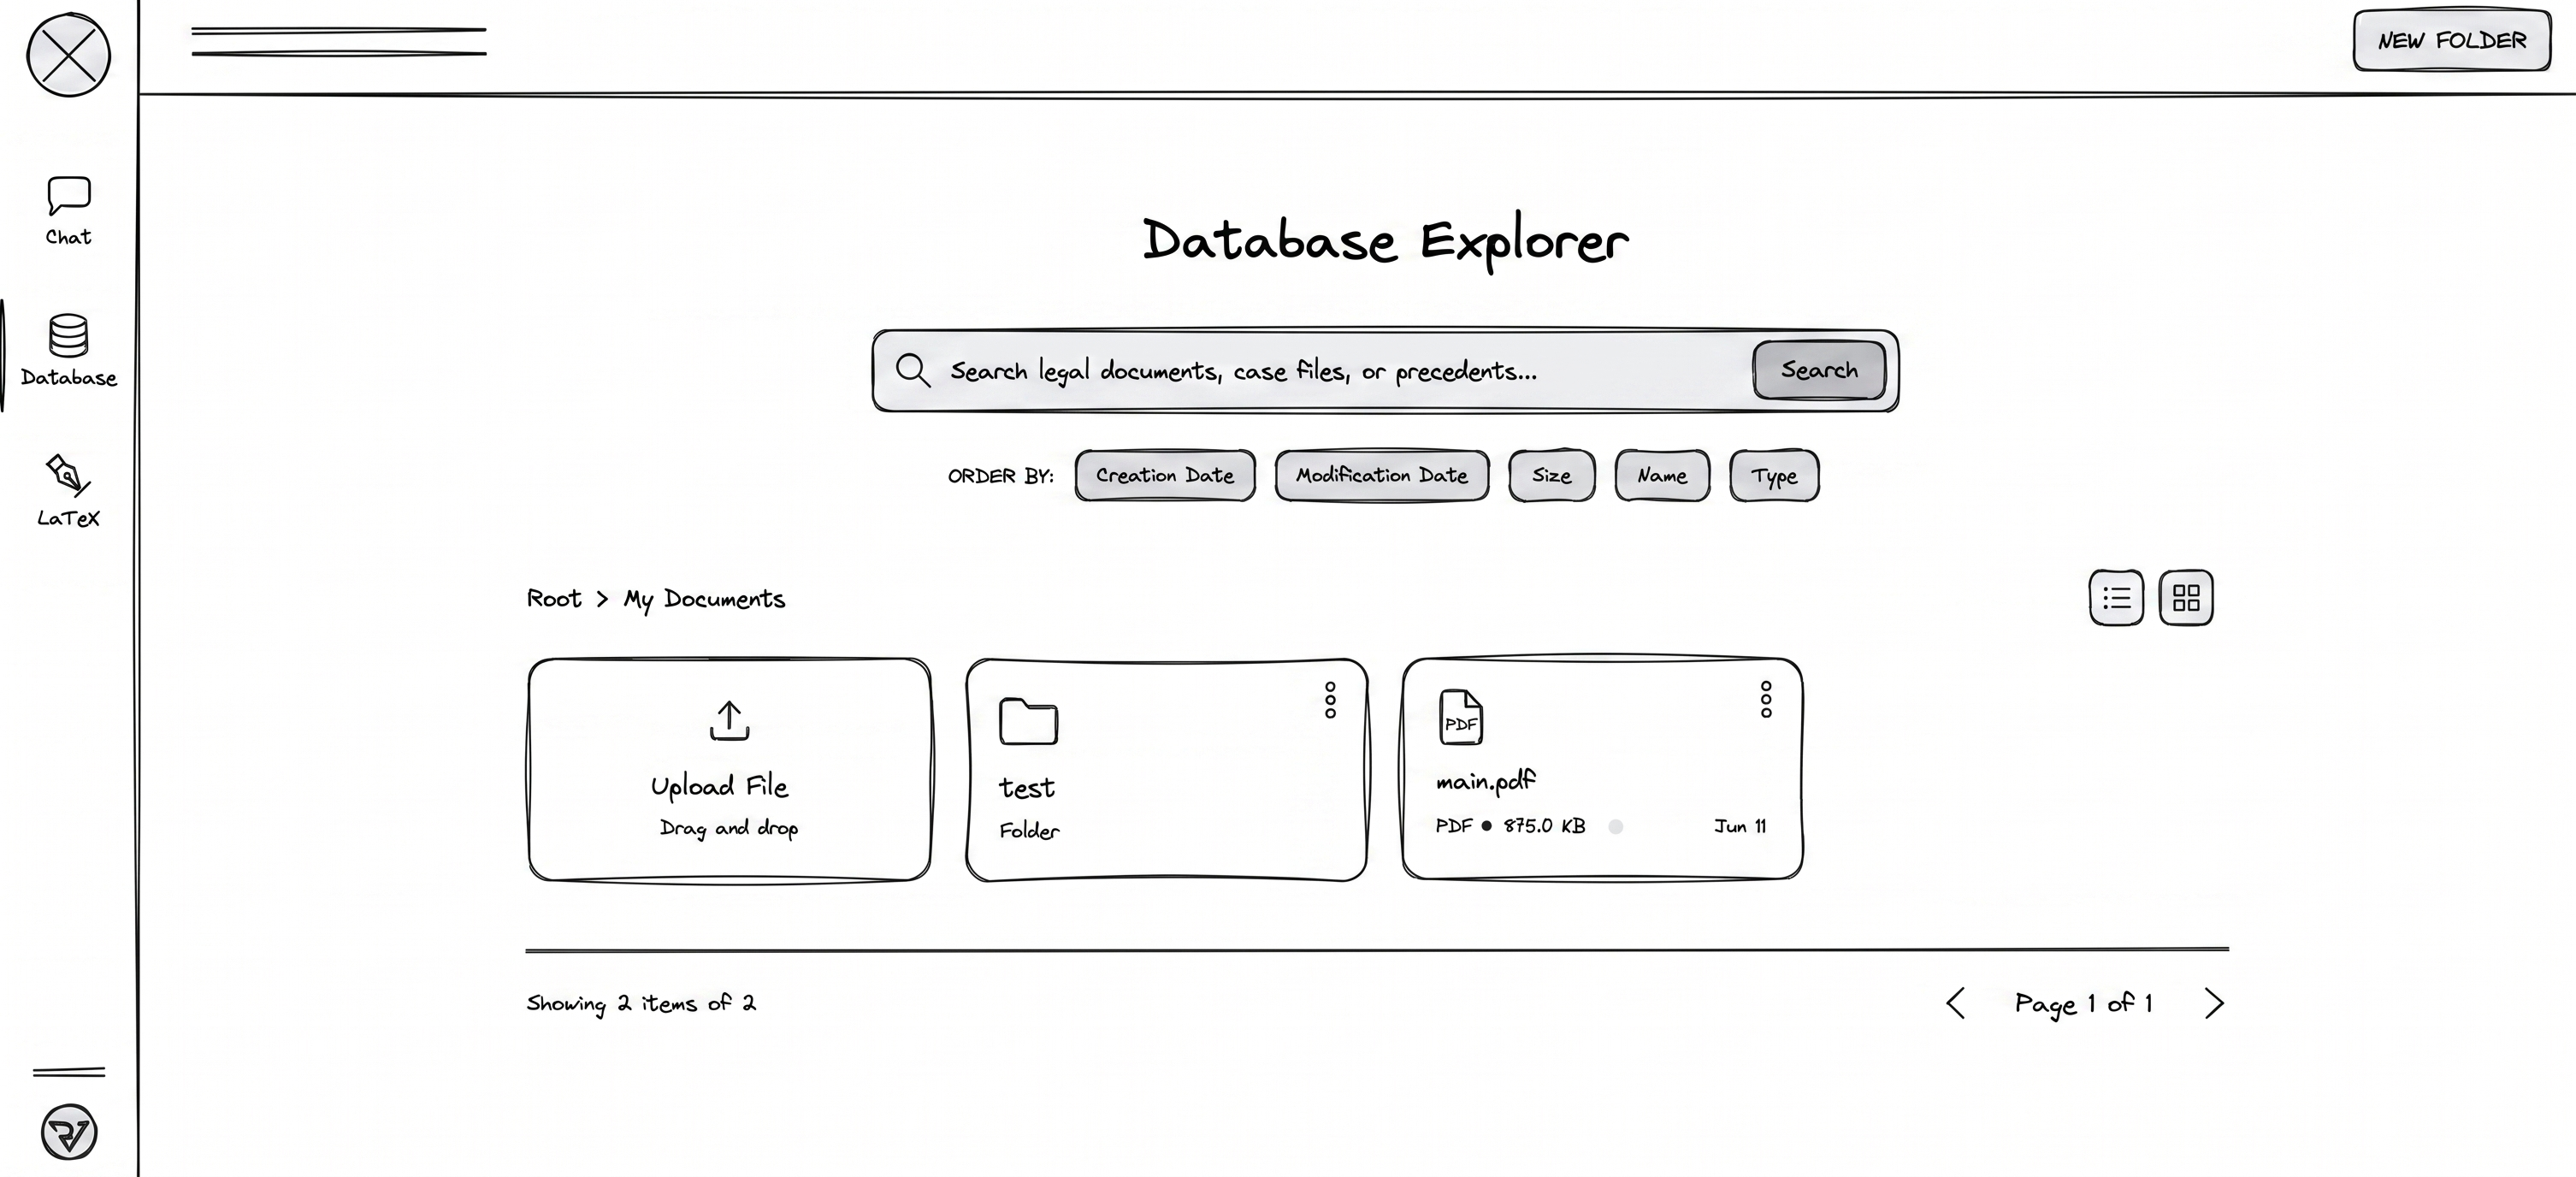
\includegraphics[width=0.9\textwidth]{Figures/fileUploads.png}
        \caption{Wireframe mockup of the Document Management System (Database Explorer)}
        \label{fig:wireframe_files}
    \end{figure}
}{}






\newpage
\section*{Conclusion}
The architecture designed for this platform successfully bridges the gap between complex legal data processing and seamless user interaction. By decoupling the heavy RAG ingestion pipeline from the main web server, implementing a robust custom logging system, and utilizing an asynchronous FastAPI backend paired with a reactive React frontend, the system achieves enterprise-grade stability and performance.
